\documentclass[12pt]{beamer}
\usepackage{../Estilos/BeamerMAF}
\usetheme{Warsaw}
\usecolortheme{seahorse}
%\useoutertheme{default}
\setbeamercovered{invisible}
% or whatever (possibly just delete it)
\setbeamertemplate{section in toc}[sections numbered]
\setbeamertemplate{subsection in toc}[subsections numbered]
\setbeamertemplate{subsection in toc}{\leavevmode\leftskip=3.2em\rlap{\hskip-2em\inserttocsectionnumber.\inserttocsubsectionnumber}\inserttocsubsection\par}
\setbeamercolor{section in toc}{fg=blue}
\setbeamercolor{subsection in toc}{fg=blue}
\setbeamercolor{frametitle}{fg=blue}
\setbeamertemplate{caption}[numbered]

\setbeamertemplate{footline}
\beamertemplatenavigationsymbolsempty
\setbeamertemplate{headline}{}


\makeatletter
\setbeamercolor{section in foot}{bg=gray!30, fg=black!90!orange}
\setbeamercolor{subsection in foot}{bg=blue!30}
\setbeamercolor{date in foot}{bg=black}
\setbeamertemplate{footline}
{
  \leavevmode%
  \hbox{%
  \begin{beamercolorbox}[wd=.333333\paperwidth,ht=2.25ex,dp=1ex,center]{section in foot}%
    \usebeamerfont{section in foot} \insertsection
  \end{beamercolorbox}%
  \begin{beamercolorbox}[wd=.333333\paperwidth,ht=2.25ex,dp=1ex,center]{subsection in foot}%
    \usebeamerfont{subsection in foot}  \insertsubsection
  \end{beamercolorbox}%
  \begin{beamercolorbox}[wd=.333333\paperwidth,ht=2.25ex,dp=1ex,right]{date in head/foot}%
    \usebeamerfont{date in head/foot} \insertshortdate{} \hspace*{2em}
    \insertframenumber{} / \inserttotalframenumber \hspace*{2ex} 
  \end{beamercolorbox}}%
  \vskip0pt%
}
\makeatother

\makeatletter
\patchcmd{\beamer@sectionintoc}{\vskip1.5em}{\vskip0.8em}{}{}
\makeatother

\newlength{\depthofsumsign}
\setlength{\depthofsumsign}{\depthof{$\sum$}}
\newcommand{\nsum}[1][1.4]{% only for \displaystyle
    \mathop{%
        \raisebox
            {-#1\depthofsumsign+1\depthofsumsign}
            {\scalebox
                {#1}
                {$\displaystyle\sum$}%
            }
    }
}
\def\scaleint#1{\vcenter{\hbox{\scaleto[3ex]{\displaystyle\int}{#1}}}}
\def\scaleoint#1{\vcenter{\hbox{\scaleto[3ex]{\displaystyle\oint}{#1}}}}
\def\bs{\mkern-12mu}

%\newcommand{\Cancel}[2][black]{{\color{#1}\cancel{\color{black}#2}}}
\makeatletter
\setbeamertemplate{footline}
{
  \leavevmode%
  \hbox{%
  \begin{beamercolorbox}[wd=.333333\paperwidth,ht=2.25ex,dp=1ex,center]{section in foot}%
    \usebeamerfont{section in foot} \insertsection
  \end{beamercolorbox}%
  \begin{beamercolorbox}[wd=.333333\paperwidth,ht=2.25ex,dp=1ex,center]{subsection in foot}%
    \usebeamerfont{subsection in foot}  \insertsubsection
  \end{beamercolorbox}%
  \begin{beamercolorbox}[wd=.333333\paperwidth,ht=2.25ex,dp=1ex,right]{date in head/foot}%
    \usebeamerfont{date in head/foot} \insertshortdate{} \hspace*{2em}
    \insertframenumber{} / \inserttotalframenumber \hspace*{2ex} 
  \end{beamercolorbox}}%
  \vskip0pt%
}
\makeatother
\date{17 de febrero de 2022}
\title{Estudiando el sistema coordenado cónico}
\subtitle{La física y la geometría}
\begin{document}
\maketitle
\fontsize{14}{14}\selectfont
\spanishdecimal{.}

\section*{Contenido}
\frame[allowframebreaks]{\frametitle{Contenido} \tableofcontents[currentsection, hideallsubsections]}

\section{Construcción de sistemas coordenados}
\frame{\tableofcontents[currentsection, hideothersubsections]}
\subsection{Introducción}

\begin{frame}
\frametitle{Introducción}
Una pregunta importante que planteamos en este momento es: ¿para qué estamos revisando los sistemas coordenados curvilíneos?
\\
\bigskip
\pause
Como respuesta presentamos la siguiente:
\end{frame}
\begin{frame}
\frametitle{Introducción}
Ante un problema de la física, debemos de seleccionar aquel sistema coordenado que mejor se adapte al problema, \emph{para aprovechar cualquier oportunidad o simetría presente en el mismo}.
\\
\bigskip
\pause
Recordemos que se modifica una expresión que modela el fenómeno, tal como una ecuación diferencial parcial.
\end{frame}
\begin{frame}
\frametitle{Introducción}
De tal manera que con el cambio de sistema coordenado, la solución completa del problema será más fácil que cuando se resuelve en un sistema cartesiano.
\end{frame}
\begin{frame}
\frametitle{Introducción}
Cuando se menciona que \enquote{es más fácil la solución}, significa que se tendrá una ecuación diferencial parcial (EDP) que puede separarse en ecuaciones diferenciales ordinarias (EDO), frecuentemente en la \enquote{forma estándar} en el nuevo sistema coordenado.
\\
\bigskip
\pause
La \emph{técnica de separación de variables}, se verá en el Tema 2 del curso.
\end{frame}

\section{Desarrollo de un sistema coordenado}
\frame{\tableofcontents[currentsection, hideothersubsections]}
\subsection{Coordenadas cónicas \texorpdfstring{$(r, \theta, \lambda)$}{(r, t, l)}.}

\begin{frame}
\frametitle{Desarrollo para un sistema especial}
A continuación veremos la manera de abordar un sistema coordenado especial, para determinar las superficies constantes, los factores de escala, los operadores diferenciales, necesarios para resolver un problema con esta geometría en particular.
\end{frame}

\subsection{Reglas de transformación}
\begin{frame}
\frametitle{Notación de índices}
Para el sistema coordenado cónico, tenemos que:
\pause
% \begin{align*}
% y^{1} = x, \hspace{1cm} y^{2} = y, \hspace{1cm} y^{3} = z
% \end{align*}
% \pause
% junto con:
\begin{align*}
q_{1} &= r \hspace{1.5cm} 0 \leq r < \infty \\[0.35em]
q_{2} &= \theta \hspace{1.5cm} b^{2} < \theta < c^{2} \\[0.35em]
q_{3} &= \lambda \hspace{1.5cm} 0 < \lambda < b^{2}
\end{align*}
donde $c^{2} > \theta^{2} > b^{2} > \lambda^{2} > 0$
\end{frame}
\begin{frame}
\frametitle{Reglas de transformación}
Las reglas de transformación son:
\pause
\begin{align*}
x &= \dfrac{r \, \theta \, \lambda}{b \, c} \\[0.5em]
y &= \dfrac{r}{b} \, \sqrt{\dfrac{(\theta^{2} - b^{2})(\lambda^{2} - b^{2})}{(b^{2} - c^{2})}} \\[0.5em]
z &= \dfrac{r}{c} \, \sqrt{\dfrac{(\theta^{2} - c^{2})(\lambda^{2} - c^{2})}{(c^{2} - b^{2})}}
\end{align*}
\end{frame}

\subsection{Superficies coordenadas}

\begin{frame}
\frametitle{Superficies coordenadas}
Para identificar las superficies constantes, elevamos al cuadrado cada lado:
\pause
\begin{align*}
x^{2} &= \dfrac{r^{2} \theta^{2} \lambda^{2}}{b^{2} c^{2}} \\[0.5em]
y^{2} &= \dfrac{r^{2}}{b^{2}} \dfrac{(\theta^{2} - b^{2})(\lambda^{2} - b^{2})}{(b^{2} - c^{2})} \\[0.5em]
z^{2} &= \dfrac{r^{2}}{c^{2}} \dfrac{(\theta^{2} - c^{2})(\lambda^{2} - c^{2})}{(c^{2} - b^{2})}
\end{align*}
\end{frame}
\begin{frame}
\frametitle{Sumando las expresiones}
Sumamos las expresiones al cuadrado:
\begin{align*}
x^{2} + y^{2} + z^{2} &= \dfrac{r^{2} \theta^{2} \lambda^{2}}{b^{2} c^{2}} + \dfrac{r^{2}}{b^{2}} \dfrac{(\theta^{2} - b^{2})(\lambda^{2} - b^{2})}{(b^{2} - c^{2})} + \\[0.5em]
&+ \dfrac{r^{2}}{c^{2}} \dfrac{(\theta^{2} - c^{2})(\lambda^{2} - c^{2})}{(c^{2} - b^{2})} =
\end{align*}
\pause
Nos armamos con paciencia para resolver la suma de fracciones, el álgebra debe de llevarse con cuidado.
\end{frame}
\begin{frame}
\frametitle{Reduciendo la expresión}\hypertarget{Suma1}
Factorizamos el término $r^{2}$:
\pause
\begin{align*}
&= r^{2} \bigg[ \dfrac{\theta^{2} \lambda^{2}}{b^{2} c^{2}} + \dfrac{1}{b^{2}} \dfrac{(\theta^{2} - b^{2})(\lambda^{2} - b^{2})}{(b^{2} - c^{2})} + \\[0.5em]
&+ \dfrac{1}{c^{2}} \dfrac{(\theta^{2} - c^{2})(\lambda^{2} - c^{2})}{(c^{2} - b^{2})} \bigg]
\end{align*}
\hyperlink{Regreso}{\beamerbutton{Regreso}}
\end{frame}
\begin{frame}
\frametitle{Analizando dos sumandos}
Nos enfocamos con los siguientes sumandos:
\pause
\begin{align*}
\dfrac{(\theta^{2} - b^{2})(\lambda^{2} - b^{2})}{b^{2}(b^{2} - c^{2})} + \dfrac{(\theta^{2} - c^{2})(\lambda^{2} - c^{2})}{c^{2}(c^{2} - b^{2})}
\end{align*}
\pause
Haciendo con cuidado el álgebra, desarrollamos cada uno de los términos:
\end{frame}
\begin{frame}
\frametitle{Desarrollando el primer término}
Entonces para el primer término:
\pause
\begin{eqnarray*}
&{}&\dfrac{(\theta^{2} - b^{2})(\lambda^{2} - b^{2})}{b^{2}(b^{2} - c^{2})} = \dfrac{\theta^{2} \lambda^{2} - \theta^2 b^{2} - \lambda^{2} b^{2} + b^{4}}{b^{2}(b^{2} - c^{2})} = \\[0.5em] \pause
&=& \dfrac{\theta^{2} \lambda^{2}}{b^{2}(b^{2} - c^{2})} - \dfrac{\theta^{2}}{(b^{2} - c^{2})} - \dfrac{\lambda^{2}}{(b^{2} - c^{2})} + \dfrac{b^{2}}{(b^{2} - c^{2})}
\end{eqnarray*}
\end{frame}
\begin{frame}
\frametitle{Desarrollando el segundo término}
Entonces para el segundo término:
\pause
\begin{eqnarray*}
&{}&\dfrac{(\theta^{2} - c^{2})(\lambda^{2} - c^{2})}{c^{2}(c^{2} - b^{2})} = \dfrac{\theta^{2} \lambda^{2} - \theta^2 c^{2} - \lambda^{2} c^{2} + c^{4}}{c^{2}(c^{2} - b^{2})} = \\[0.5em] \pause
&=& \dfrac{\theta^{2} \lambda^{2}}{c^{2}(c^{2} - b^{2})} - \dfrac{\theta^{2}}{(c^{2} - b^{2})} - \dfrac{\lambda^{2}}{(c^{2} - b^{2})} + \dfrac{c^{2}}{(c^{2} - b^{2})}
\end{eqnarray*}
\end{frame}
\begin{frame}
\frametitle{Sumando los dos términos}
Ordenando y sumando los dos términos, tendremos:
\pause
\begin{align*}
&\dfrac{\theta^{2} \lambda^{2}}{b^{2}(b^{2} - c^{2})} + \dfrac{\theta^{2} \lambda^{2}}{c^{2}(c^{2} - b^{2})} - \dfrac{\theta^{2}}{(b^{2} - c^{2})} - \dfrac{\theta^{2}}{(c^{2} - b^{2})} + \\[0.5em] 
&- \dfrac{\lambda^{2}}{(b^{2} - c^{2})} - \dfrac{\lambda^{2}}{(c^{2} - b^{2})} + \dfrac{b^{2}}{(b^{2} - c^{2})} + \dfrac{c^{2}}{(c^{2} - b^{2})}
\end{align*}
\end{frame}
\begin{frame}
\frametitle{Reduciendo los términos}
Del primero término encontrado, vemos que:
\pause
\begin{eqnarray*}
&{}&\dfrac{\theta^{2} \lambda^{2}}{b^{2}(b^{2} - c^{2})} + \dfrac{\theta^{2} \lambda^{2}}{c^{2}(c^{2} - b^{2})} = \\[0.5em] \pause
&=& \dfrac{\theta^{2} \lambda^{2} c^{2} (c^{2} - b^{2}) + \theta^{2} \lambda^{2} b^{2} (b^{2} - c^{2})}{b^{2} c^{2}(b^{2} - c^{2})(c^{2} - b^{2})} = \\[0.5em] \pause
&=& \dfrac{\theta^{2} \lambda^{2} \big[ c^{2} (c^{2} - b^{2}) + b^{2} (b^{2} - c^{2}) \big]}{b^{2} c^{2}(b^{2} - c^{2})(c^{2} - b^{2})} = \\[0.5em] \pause
&=& \dfrac{\theta^{2} \lambda^{2} (c^{4} - b^{2} c^{2} + b^{4} -b^{2} c^{2})}{-b^{2} c^{2} (b^{2} - c^{2})^{2}} = \pause - \dfrac{\theta^{2} \lambda^{2}}{b^{2} c^{2}} \Cancel[red]{\dfrac{(b^{2} - c^{2})^{2}}{(b^{2} - c^{2})^{2}}} =
\end{eqnarray*}
\end{frame}
\begin{frame}
\frametitle{Resultado reducido}
Entonces el resultado:
\pause
\begin{align*}
\dfrac{\theta^{2} \lambda^{2}}{b^{2}(b^{2} - c^{2})} + \dfrac{\theta^{2} \lambda^{2}}{c^{2}(c^{2} - b^{2})} = - \dfrac{\theta^{2} \lambda^{2}}{b^{2} c^{2}}
\end{align*}
\pause
Quedando pendientes los otros términos de la suma.
\end{frame}
\begin{frame}
\frametitle{Los otros resultados}
Es fácil revisar que:
\pause
\begin{eqnarray*}
- \dfrac{\theta^{2}}{(b^{2} {-} c^{2})} {-} \dfrac{\theta^{2}}{(c^{2} {-} b^{2})} &=& + \dfrac{\theta^{2}}{(c^{2} {-} b^{2})} {-} \dfrac{\theta^{2}}{(c^{2} {-} b^{2})} = 0 \\[0.5em] \pause
- \dfrac{\lambda^{2}}{(b^{2} {-} c^{2})} {-} \dfrac{\lambda^{2}}{(c^{2} {-} b^{2})} &=& + \dfrac{\lambda^{2}}{(c^{2} {-} b^{2})} {-} \dfrac{\lambda^{2}}{(c^{2} {-} b^{2})} = 0
\end{eqnarray*}
\end{frame}
\begin{frame}
\frametitle{Por último}
El último término que queda es:
\pause
\begin{eqnarray*}
\begin{aligned}
\dfrac{b^{2}}{(b^{2} - c^{2})} + \dfrac{c^{2}}{(c^{2} - b^{2})} &= \pause \dfrac{b^{2}}{(b^{2} - c^{2})} - \dfrac{c^{2}}{(b^{2} - c^{2})} = \\[0.5em] \pause
&= \Cancel[red]{\dfrac{(b^{2} - c^{2})}{(b^{2} - c^{2})}} = 1
\end{aligned}
\end{eqnarray*}
\end{frame}  
\begin{frame}
\frametitle{La suma completa}\hypertarget{Suma2}
Hemos llegado entonces a que la suma completa es:
\begin{eqnarray*}
x^{2} + y^{2} + z^{2} &=& \pause r^{2} \bigg[ \Cancel[blue]{\dfrac{\theta^{2} \lambda^{2}}{b^{2} c^{2}}} - \Cancel[blue]{\dfrac{\theta^{2} \lambda^{2}}{b^{2} c^{2}}} + 1 \bigg] = \\[0.5em] \pause
x^{2} + y^{2} + z^{2} &=& r^{2}
\end{eqnarray*}
\pause
Que nos definen una familia de esferas concéntricas de radio $r$, siendo la primera superficie coordenada en este sistema cónico.
\hyperlink{Regreso}{\beamerbutton{Regreso}}
\end{frame}
\begin{frame}
\frametitle{Superficie coordenada con $r$ constante}
\begin{figure}
  \centering
  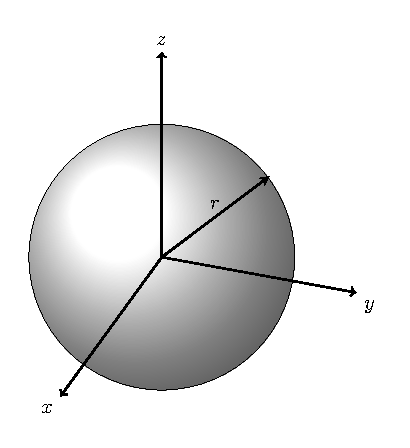
\includegraphics[scale=1]{Imagenes/Sistema_Conico_Superficie_Constante_01.eps}
\end{figure}
\end{frame}
\begin{frame}
\frametitle{Superficie coordenada con $\theta$ constante}
Al dejar que $\theta$ sea constante, y como $\theta > 0$, podemos revisar lo siguiente:
\pause
\begin{align*}
\dfrac{x^{2}}{\theta^{2}} + \dfrac{y^{2}}{\theta^{2} - b^{2}} + \dfrac{z^{2}}{\theta^{2} - c^{2}} = 0
\end{align*}
\pause
Nos define una familia de conos, que es la segunda superficie coordenada.
\end{frame}
\begin{frame}
\frametitle{Superficie coordenada con $\lambda$ constante}
Ahora hacemos que $\lambda$ sea constante, y como $\lambda > 0$, podemos revisar lo siguiente:
\pause
\begin{align*}
\dfrac{x^{2}}{\lambda^{2}} + \dfrac{y^{2}}{\lambda^{2} - b^{2}} + \dfrac{z^{2}}{\lambda^{2} - c^{2}} = 0
\end{align*}
\pause
Nos define otra familia de conos, que es la tercera superficie coordenada.
\end{frame}
\begin{frame}
\frametitle{Intersección de las superficies}
\begin{figure}
  \centering
  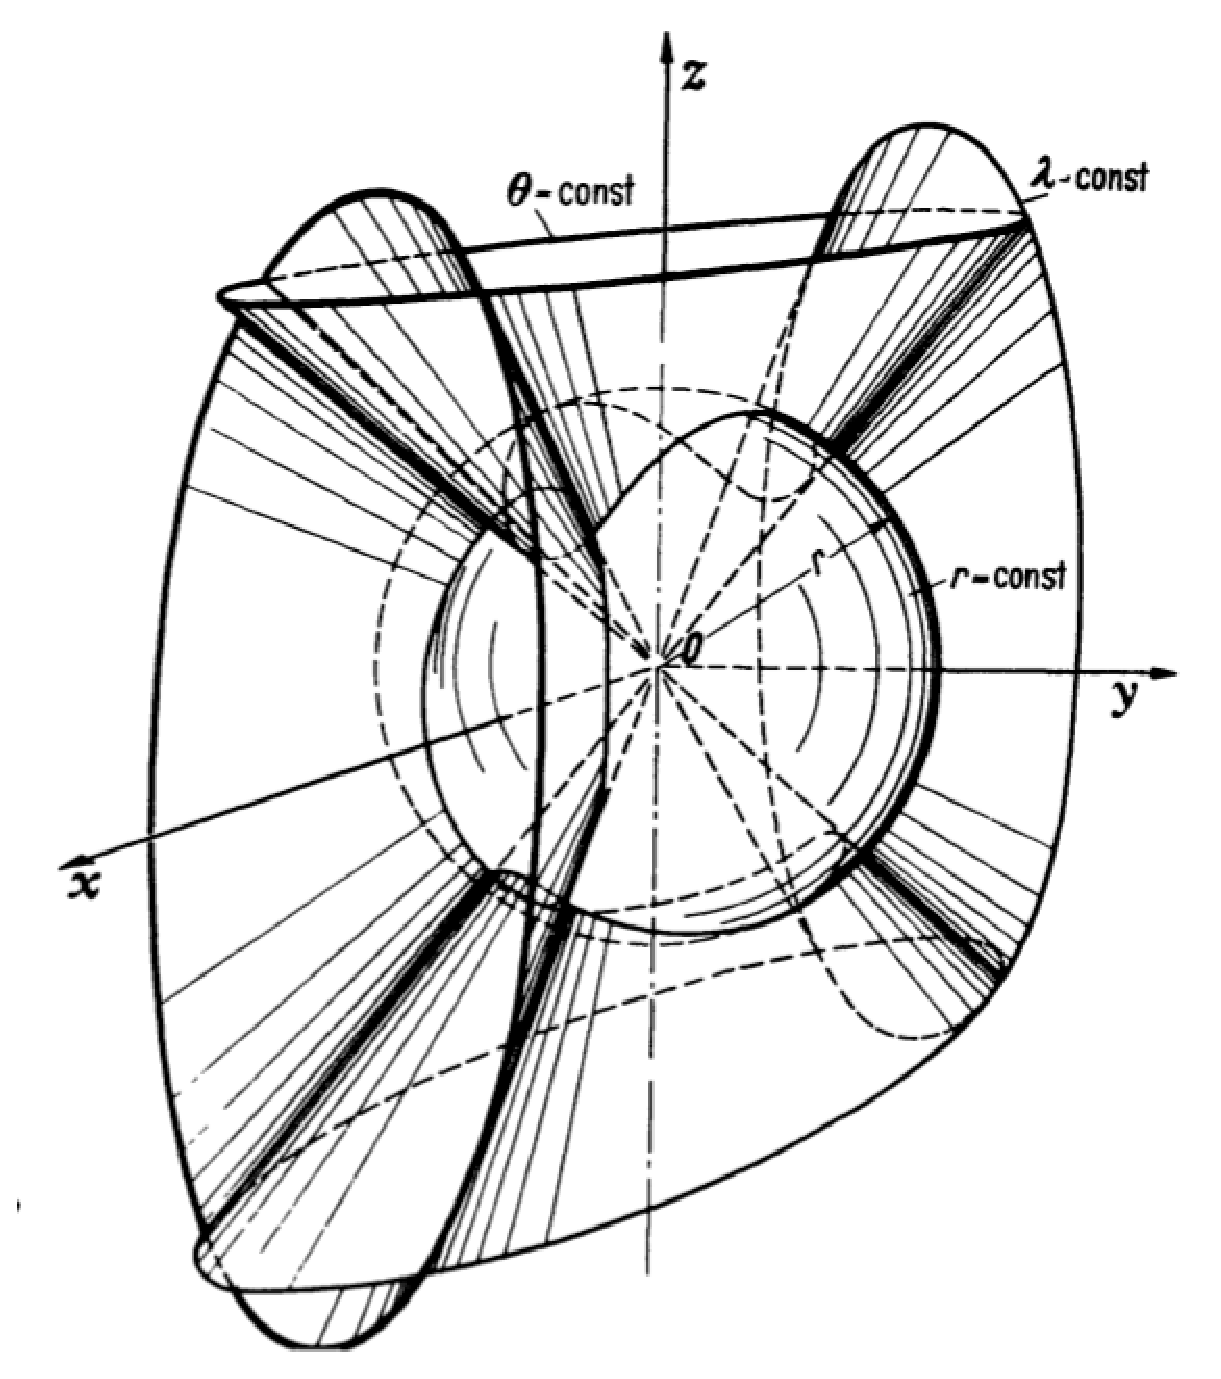
\includegraphics[scale=0.3]{Imagenes/Sistema_Conico.eps}
\end{figure}
\end{frame}

%\subsection{Tensor métrico}
\subsection{Factores de escala}

% \begin{frame}
% \frametitle{Calculando el tensor métrico}
% El siguiente paso es determinar las componentes del tensor métrico asociado al sistema coordenado cónico.
% \\
% \bigskip
% \pause
% \begin{align*}
% g_{ij} = \pdv{y^{m}}{x^{i}} \, \pdv{y^{m}}{x^{j}} \hspace{1cm} i, j \quad \mbox{ índices libres}
% \end{align*}
% \end{frame}
% \begin{frame}
% \frametitle{Las componentes métricas}
% Entonces:
% \pause
% \begin{align*}
% &g_{11} = \left( \dfrac{\theta \lambda}{b c} \right) \left( \dfrac{\theta \lambda}{b c} \right) + \\[0.5em] 
% &+ \left( \dfrac{1}{b} \sqrt{\dfrac{(\theta^{2} {-} b^{2})(\lambda^{2} {-} b^{2})}{(b^{2} {-} c^{2})}} \right) \left( \dfrac{1}{b} \sqrt{\dfrac{(\theta^{2} {-} b^{2})(\lambda^{2} {-} b^{2})}{(b^{2} {-} c^{2})}} \right) + \\[0.5em] 
% &+ \left( \dfrac{1}{c} \sqrt{\dfrac{(\theta^{2} {-} c^{2})(\lambda^{2} {-} c^{2})}{(c^{2} {-} b^{2})}} \right) \left( \dfrac{1}{c} \sqrt{\dfrac{(\theta^{2} {-} c^{2})(\lambda^{2} {-} c^{2})}{(c^{2} {-} b^{2})}} \right)
% \end{align*}
% \end{frame}
% \begin{frame}
% \frametitle{De nuevo con el álgebra}
% Por lo que:
% \pause
% \begin{align*}
% g_{11} &= \left( \dfrac{\theta^{2} \lambda^{2}}{b^{2} c^{2}} \right) + \dfrac{1}{b^{2}} \dfrac{(\theta^{2} {-} b^{2})(\lambda^{2} {-} b^{2})}{(b^{2} {-} c^{2})} + \\[0.5em] 
% &+ \dfrac{1}{c^{2}} \dfrac{(\theta^{2} {-} c^{2})(\lambda^{2} {-} c^{2})}{(c^{2} {-} b^{2})}
% \end{align*}
% \pause
% De donde ya conocemos el resultado los dos términos de la suma, por lo que se reducen las operaciones para esta componente métrica.
% \end{frame}
% \begin{frame}
% \frametitle{La componente $g_{11}$}
% Entonces el valor es:
% \pause
% \begin{eqnarray*}
% g_{11} &=& \left( \dfrac{\theta^{2} \lambda^{2}}{b^{2} c^{2}} \right) - \left( \dfrac{\theta^{2} \lambda^{2}}{b^{2} c^{2}} \right) + 1 = \\[0.5em] \pause
% g_{11} &=& 1
% \end{eqnarray*}
% \end{frame}
% \begin{frame}
% \frametitle{Componentes métricas nulas}
% Una tarea que se debe de realizar en cualquier ejercicio en el curso, es \emph{calcular explícitamente} cada una de las componentes del tensor métrico.
% \\
% \bigskip
% \pause
% Siendo cierto que fuera de la diagonal principal, las componentes son nulas, pero no por ello debemos de evitar el ejercicio y práctica.
% \end{frame}
% \begin{frame}
% \frametitle{Las componentes $g_{22}$ y $g_{33}$}
% Para las otras componentes no nulas, se tiene que:
% \pause
% \begin{align*}
% g_{22} &= \dfrac{r^{2} (\theta^{2} - \lambda^{2})}{(\theta^{2} - b^{2})(c^{2} - \theta^{2})} \\[0.5em]
% g_{33} &= \dfrac{r^{2} (\theta^{2} - \lambda^{2})}{(\lambda^{2} - b^{2})(\lambda^{2} - c^{2})}
% \end{align*}
% \end{frame}
% \begin{frame}
% \frametitle{El tensor métrico}
% El tensor métrico asociado al sistema coordenado cónico es:
% \pause
% \begin{align*}
% g_{ij} = \mqty(
% 1 & 0 & 0 \\
% 0 & \dfrac{r^{2} (\theta^{2} - \lambda^{2})}{(\theta^{2} - b^{2})(c^{2} - \theta^{2})} & 0 \\
% 0 & 0 & \dfrac{r^{2} (\theta^{2} - \lambda^{2})}{(\lambda^{2} - b^{2})(\lambda^{2} - c^{2})}
% )
% \end{align*}
% \end{frame}

% \subsection{Factores de escala}

\begin{frame}
\frametitle{Los factores de escala}
Para obtener los factores de escala, ocupamos la expresión:
\pause
\begin{eqnarray*}
h_{i} = \pause \abs{\dv{\vb{r}}{u_{i}}} = \pause \sqrt{\bigg( \pdv{x}{u_{i}} \bigg)^{2} + \bigg( \pdv{y}{u_{i}} \bigg)^{2} + \bigg( \pdv{z}{u_{i}} \bigg)^{2}}
\end{eqnarray*}
\end{frame}
\begin{frame}
\frametitle{Obteniendo $h_{r}$}
Para obtener el factor de escala $h_{r}$, debemos de calcular:
\pause
\begin{align*}
h_{r} = \sqrt{\bigg( \pdv{x}{r} \bigg)^{2} + \bigg( \pdv{y}{r} \bigg)^{2} + \bigg( \pdv{z}{r} \bigg)^{2}}
\end{align*}
\end{frame}
\begin{frame}
\frametitle{Las derivadas parciales 1}
Desarrollamos de manera explícita las derivadas parciales:
\pause
\begin{eqnarray*}
\begin{aligned}
\pdv{x}{r} &= \pause \displaystyle \pdv{r} \bigg( \dfrac{r \theta \lambda}{b c} \bigg) = \pause \dfrac{\theta \lambda}{b c} \\[0.5em] \pause
\Rightarrow \hspace{0.3cm} \bigg( \pdv{x}{r} \bigg)^{2} &= \dfrac{\theta^{2} \lambda^{2}}{b^{2} c^{2}}
\end{aligned}
\end{eqnarray*}
\end{frame}
\begin{frame}
\frametitle{Las derivadas parciales 2}
\begin{eqnarray*}
\begin{aligned}
\pdv{y}{r} &= \pause \pdv{r} \bigg( \dfrac{r}{b} \sqrt{\dfrac{ (\theta^{2} - b^{2}) (\lambda^{2} - b^{2}) }{(b^{2} - c^{2})}} \bigg) = \\[0.5em] \pause
&= \dfrac{1}{b} \sqrt{\dfrac{ (\theta^{2} - b^{2}) (\lambda^{2} - b^{2}) }{(b^{2} - c^{2})}} \\[0.5em] \pause
\Rightarrow \hspace{0.3cm} \bigg( \pdv{y}{r} \bigg)^{2} &= \dfrac{1}{b^{2}} \dfrac{ (\theta^{2} - b^{2}) (\lambda^{2} - b^{2})}{(b^{2} - c^{2})}
\end{aligned}
\end{eqnarray*}
\end{frame}
\begin{frame}
\frametitle{Las derivadas parciales 3}
\begin{eqnarray*}
\begin{aligned}
\pdv{z}{r} &= \pause \pdv{r} \bigg( \dfrac{r}{c} \sqrt{\dfrac{ (\theta^{2} - c^{2}) (\lambda^{2} - c^{2}) }{(c^{2} - b^{2})}} \bigg) = \\[0.5em] \pause
&= \dfrac{1}{c} \sqrt{\dfrac{ (\theta^{2} - c^{2}) (\lambda^{2} - c^{2}) }{(c^{2} - b^{2})}} \\[0.5em] \pause
\Rightarrow \hspace{0.3cm} \bigg( \pdv{z}{r} \bigg)^{2} &= \dfrac{1}{c^{2}} \dfrac{ (\theta^{2} - c^{2}) (\lambda^{2} - c^{2}) }{(c^{2} - b^{2})}
\end{aligned}
\end{eqnarray*}
\end{frame}
\begin{frame}
\frametitle{Haciendo la suma de las derivadas parciales}
Podemos hacer la suma:
\pause
\begin{align*}
\bigg( \pdv{x}{r} \bigg)^{2} + \bigg( \pdv{y}{r} \bigg)^{2} + \bigg( \pdv{z}{r} \bigg)^{2} =
\end{align*}
Entonces:
\pause
\begin{align*}
\dfrac{\theta^{2} \lambda^{2}}{b^{2} c^{2}} + \dfrac{1}{b^{2}} \dfrac{ (\theta^{2} - b^{2}) (\lambda^{2} - b^{2})}{(b^{2} - c^{2})} + \dfrac{1}{c^{2}} \dfrac{ (\theta^{2} - c^{2}) (\lambda^{2} - c^{2}) }{(c^{2} - b^{2})}
\end{align*}
\hypertarget{Regreso}
Esta suma ya se realizó: \hyperlink{Suma1}{\beamerbutton{Suma}} \hspace{1.5cm} \hyperlink{Suma2}{\beamerbutton{Resultado}}
\end{frame}
\begin{frame}
\frametitle{El factor de escala $h_{r}$}
Entonces tenemos que:
\pause
\begin{align*}
h_{r} &= \sqrt{\bigg( \pdv{x}{r} \bigg)^{2} + \bigg( \pdv{y}{r} \bigg)^{2} + \bigg( \pdv{z}{r} \bigg)^{2}} = \\[0.5em]
&= 1
\end{align*}
\end{frame}
\begin{frame}
\frametitle{El factor de escala $h_{\theta}$}
Ocupamos nuevamente la expresión para obtener el factor de escala $h_{\theta}$:
\pause
\begin{align*}
h_{\theta} &= \sqrt{\bigg( \pdv{x}{\theta} \bigg)^{2} + \bigg( \pdv{y}{\theta} \bigg)^{2} + \bigg( \pdv{z}{\theta} \bigg)^{2}}
\end{align*}
Recomendamos hacer el cálculo de las derivadas parciales de manera paulatina, para evitar errores.
\end{frame}
\begin{frame}
\frametitle{La derivada parcial $\pdv*{x}{\theta}$}
Comenzamos con:
\pause
\begin{eqnarray*}
\begin{aligned}
\pdv{x}{\theta} &= \pause \displaystyle \pdv{\theta} \bigg( \dfrac{r \theta \lambda}{b c} \bigg) = \pause \dfrac{r \lambda}{b c} \\[0.5em] \pause
\Rightarrow \hspace{0.3cm} \bigg( \pdv{x}{\theta} \bigg)^{2} &= \dfrac{r^{2} \lambda^{2}}{b^{2} c^{2}}
\end{aligned}
\end{eqnarray*}
\end{frame}
\begin{frame}
\frametitle{La derivada parcial $\pdv*{y}{\theta}$}
\begin{eqnarray*}
\begin{aligned}
\pdv{y}{\theta} &= \pause \pdv{\theta} \bigg( \dfrac{r}{b} \sqrt{\dfrac{ (\theta^{2} - b^{2}) (\lambda^{2} - b^{2}) }{(b^{2} - c^{2})}} \bigg) = \\[0.5em] \pause
&= \dfrac{r \theta (\lambda^{2} - b^{2})}{b (b^{2} -c^{2}) \bigg[ \dfrac{(\theta^{2} - b^{2})(\lambda^{2} - b^{2})}{(b^{2} - c^{2})} \bigg]^{\frac{1}{2}}}
\end{aligned}
\end{eqnarray*}  
\end{frame}
\begin{frame}
\frametitle{La derivada parcial $\pdv*{y}{\theta}$}
\begin{eqnarray*}
\begin{aligned}
\Rightarrow \hspace{0.3cm} \bigg( \pdv{y}{\theta} \bigg)^{2} &= \dfrac{r^{2} \theta^{2} (\lambda^{2} - b^{2})^{2}}{b^{2} (b^{2} -c^{2})^{2} \bigg[ \dfrac{(\theta^{2} - b^{2})(\lambda^{2} - b^{2})}{(b^{2} - c^{2})} \bigg]} = \\[0.5em] \pause
&= \dfrac{r^{2} \theta^{2} (\lambda^{2} - b^{2})}{b^{2} (b^{2} - c^{2}) (\theta^{2} - b^{2})}
\end{aligned}
\end{eqnarray*}  
\end{frame}
\begin{frame}
\frametitle{La derivada parcial $\pdv*{z}{\theta}$}
Para la tercera derivada parcial:
\pause
\begin{eqnarray*}
\begin{aligned}
\pdv{z}{\theta} &= \pause \pdv{\theta} \bigg( \dfrac{r}{c} \sqrt{\dfrac{(\theta^{2} - c^{2})(\lambda^{2} - c^{2})}{(c^{2} - b^{2})}} \bigg) = \\[0.5em] \pause
&= \dfrac{r \theta (\lambda^{2} - c^{2})}{c (c^{2} - b^{2}) \bigg[ \dfrac{(\theta^{2} - c^{2})(\lambda^{2} - c^{2})}{(c^{2} - b^{2})} \bigg]^{\frac{1}{2}}}
\end{aligned}
\end{eqnarray*}
\end{frame}
\begin{frame}
\frametitle{La derivada parcial $\pdv*{z}{\theta}$}
\begin{eqnarray*}
\begin{aligned}
\Rightarrow \hspace{0.3cm} \bigg( \pdv{z}{\theta} \bigg)^{2} &= \dfrac{r^{2} \theta^{2} (\lambda^{2} - c^{2})^{2}}{c^{2} (c^{2} - b^{2})^{2} \bigg[ \dfrac{(\theta^{2} - c^{2})(\lambda^{2} - c^{2})}{(c^{2} - b^{2})} \bigg]} = \\[0.5em] \pause
&= \dfrac{r^{2} \theta^{2} (\lambda^{2} - c^{2})^{2}}{c^{2} (c^{2} - b^{2}) (\theta^{2} - c^{2})}
\end{aligned}
\end{eqnarray*}
\end{frame}
\begin{frame}
\frametitle{Sumando las derivadas parciales}
Al sumar las tres derivadas parciales, se tiene que:
\pause
\begin{eqnarray*}
\begin{aligned}
h_{\theta} &= \sqrt{\bigg( \pdv{x}{\theta} \bigg)^{2} + \bigg( \pdv{y}{\theta} \bigg)^{2} + \bigg( \pdv{z}{\theta} \bigg)^{2}} = \\[0.5em] \pause
&= \dfrac{r^{2} \lambda^{2}}{b^{2} c^{2}} {+} \dfrac{r^{2} \theta^{2} (\lambda^{2} - b^{2})}{b^{2} (b^{2} - c^{2}) (\theta^{2} - b^{2})} {+} \dfrac{r^{2} \theta^{2} (\lambda^{2} - c^{2})^{2}}{c^{2} (c^{2} - b^{2}) (\theta^{2} - c^{2})}
\end{aligned}
\end{eqnarray*}
\end{frame}
\begin{frame}
\frametitle{El factor de escala $h_{\theta}$}
Luego de un cuidadoso trabajo algebraico, se llega al resultado:
\pause
\begin{align*}
h_{\theta} = r \sqrt{\dfrac{(\theta^{2} - \lambda^{2})}{(\theta^{2} - b^{2})(c^{2} - \theta^{2})}}
\end{align*}
\end{frame}
\begin{frame}
\frametitle{El factor de escala $h_{\lambda}$}
Siguiendo el mismo procedimiento, el tercer factor de escala para este sistema coordenado cónico es:
\pause
\begin{align*}
h_{\lambda} = r \sqrt{\dfrac{(\theta^{2} - \lambda^{2})}{(\lambda^{2} - b^{2})(\lambda^{2} - c^{2})}}
\end{align*}
\pause
En las soluciones de los ejercicios a cuenta y del examen, se debe de hacer todo el procedimiento de manera explícita.
\end{frame}
\begin{frame}
\frametitle{Los factores de escala}
Hemos calculado los factores de escala:
\pause
\begin{align*}
h_{r} &= 1 \\[0.5em]
h_{\theta} &=  r \, \sqrt{\dfrac{(\theta^{2} - \lambda^{2})}{(\theta^{2} - b^{2})(c^{2} - \theta^{2})}} \\[0.5em]
h_{\lambda} &= r \, \sqrt{\dfrac{(\theta^{2} - \lambda^{2})}{(\lambda^{2} - b^{2})(\lambda^{2} - c^{2})}}
\end{align*}
\end{frame}

\section{Diferencial de desplazamiento}
\frame{\tableofcontents[currentsection, hideothersubsections]}
\subsection{Vectores unitarios en el sistema cónico}

\begin{frame}
\frametitle{Vectores unitarios}
De acuerdo con las notas de trabajo, los vectores unitarios se expresan como:
\pause
\begin{align*}
\vu{e}_{i} = \dfrac{1}{h_{i}} \, \pdv{\vb{r}}{u_{i}}
\end{align*}
\end{frame}

\subsection{Diferencial de desplazamiento}

\begin{frame}
\frametitle{Obteniendo el diferencial}
El cuadrado de la distancia entre dos puntos está dado por:
\pause
\begin{align*}
\big( \dd{s} \big)^{2} = \big( h_{1} \dd{q_{1}} \big)^{2} + \big( h_{2} \dd{q_{2}} \big)^{2} + \big( h_{3} \dd{q_{3}} \big)^{2}
\end{align*}
\end{frame}
\begin{frame}
\frametitle{Estimado el diferencial de desplazamiento}
Una vez que se cuenta con los factores de escala, podemos expresar el diferencial de desplazamiento en el sistema coordenado cónico:
\pause
\begin{align*}
&\big( \dd{s} \big)^{2} = \big( \dd{r} \big)^{2} + \\[0.5em]
&+ r^{2} \big( \theta^{2} {-} \lambda^{2} \big) \bigg[ \dfrac{(\dd{\theta})^{2}}{(\theta^{2} {-} b^{2})(c^{2} {-} \theta^{2})} {+} \dfrac{(\dd{\lambda})^{2}}{(b^{2} {-} \lambda^{2})(c^{2} {-} \lambda^{2})} \bigg]
\end{align*}
\end{frame}
\begin{frame}
\frametitle{Obteniendo más elementos del sistema coordenado}
Los factores de escala pueden identificarse convenientemente mediante la relación:
\pause
\begin{align*}
\dd{s_{i}} = h_{i} \dd{q_{i}}
\end{align*}
para cualquier $\dd{q_{i}}$, conservando las otras $q$ constantes.
\end{frame}
\begin{frame}
\frametitle{Elementos de área y de volumen}
Con lo anterior, se pueden desarrollar los elementos de área y volumen:
\pause
\begin{eqnarray*}
\begin{aligned}
\dd{\sigma_{ij}} &= \dd{s_{i}} \dd{s_{j}} = h_{i} \, h_{j} \dd{q_{i}} \dd{q_{j}} \\[0.5em] \pause
\dd{\tau} &= \dd{s_{1}} \dd{s_{2}} \dd{s_{3}}= h_{1} \, h_{2} \, h_{3} \dd{q_{1}} \dd{q_{2}} \dd{q_{3}}
\end{aligned}
\end{eqnarray*}
\end{frame}

% \section{Operadores diferenciales}
% \frame{\tableofcontents[currentsection, hideothersubsections]}

% \subsection{Gradiente}

% \begin{frame}
% \frametitle{El gradiente}
% En un sistema coordenado generalizado $(x^{1}, x^{2}, x^{3})$, escribimos el gradiente de una función escalar $\phi$ como:
% \pause
% \begin{align*}
% \grad{\phi} = \dfrac{1}{(g_{11})^{\frac{1}{2}}} \, \vu{e}_{1} \, \pdv{\phi}{x^{1}} + \dfrac{1}{(g_{22})^{\frac{1}{2}}} \, \vu{e}_{2} \, \pdv{\phi}{x^{2}} + \dfrac{1}{(g_{33})^{\frac{1}{2}}} \, \vu{e}_{3} \, \pdv{\phi}{x^{3}}
% \end{align*}
% \end{frame}

% \subsection{Divergencia}

% \begin{frame}
% \frametitle{La divergencia}
% La divergencia de un vector $\vb{B}$ se expresa como:
% \pause
% \begin{align*}
% \div{\vb{B}} &= g^{\frac{1}{2}} \, \left\{ \pdv{x^{1}} \left[ \left( \dfrac{g}{g_{11}} \right)^{\frac{1}{2}} B_{1} \right] {+} \pdv{x^{2}} \left[ \left( \dfrac{g}{g_{22}} \right)^{\frac{1}{2}} B_{2} \right] + \right. \\[0.5em] 
% &+ \left. \pdv{x^{3}} \left[ \left( \dfrac{g}{g_{33}} \right)^{\frac{1}{2}} B_{3} \right] \right\}
% \end{align*}
% \end{frame}

% \subsection{Rotacional}

% \begin{frame}
% \frametitle{El rotacional}
% El rotacional de un vector $\vb{B}$ es:
% \pause
% \begin{align*}
% \curl{B} = \mqty|
% \vu{e}_{1} \left( \dfrac{g_{11}}{g} \right)^{\frac{1}{2}} & \vu{e}_{2} \left( \dfrac{g_{22}}{g} \right)^{\frac{1}{2}} & \vu{e}_{3} \left( \dfrac{g_{33}}{g} \right)^{\frac{1}{2}} \\[1em]
% \displaystyle \pdv{x^{1}} & \displaystyle \pdv{x^{2}} & \displaystyle \pdv{x^{3}} \\[1em]
% (g_{11})^{\frac{1}{2}} B_{1} & (g_{22})^{\frac{1}{2}} B_{2} & (g_{33})^{\frac{1}{2}} B_{3}
% |
% \end{align*}
% \end{frame}

% \subsection{Laplaciano}

% \begin{frame}
% \frametitle{El Laplaciano}
% El Laplaciano en un sistema coordenado generalizado, se define por la expresión:
% \pause
% \begin{align*}
% \laplacian{\varphi} = g^{-\frac{1}{2}} \nsum_{i=1}^{3} \pdv{x^{i}} \bigg[ \dfrac{g^{\frac{1}{2}}}{g_{ii}} \, \pdv{\varphi}{x^{i}}\bigg]
% \end{align*}
% \end{frame}

% \section{Aplicación: La ecuación de Helmholtz}
% \frame{\tableofcontents[currentsection, hideothersubsections]}
% \subsection{Construyendo la ecuación}

% \begin{frame}
% \frametitle{La ecuación de Helmholtz}
% Sabemos que la ecuación de Helmholtz se expresa por:
% \pause
% \begin{align*}
% \laplacian{E} + k \, E = 0
% \end{align*}
% donde $k$ es el número de onda, $E$ es la función escalar que es solución a la ecuación.
% \\
% \bigskip
% \pause
% Expresemos esta ecuación en el sistema coordenado cónico.
% \end{frame}
% \begin{frame}
% \frametitle{El Laplaciano en coord. cónicas}
% Ya conocemos la expresión para el Laplaciano en coordenadas generalizadas:
% \begin{align*}
% \laplacian{\varphi} = g^{-\frac{1}{2}} \nsum_{i=1}^{3} \pdv{x^{i}} \bigg[ \dfrac{g^{\frac{1}{2}}}{g_{ii}} \, \pdv{\varphi}{x^{i}}\bigg]
%   \end{align*}
% \pause
% Por lo que hay que calcular algunos valores de manera anticipada.  
% \end{frame}
% \begin{frame}
% \frametitle{Simplificando las operaciones}
% Con la finalidad de simplificar las operaciones, hagamos que:
% \pause
% \begin{align*}
% f(\theta) &= \sqrt{(\theta^{2} - b^{2})(c^{2} - \theta^{2})} \\[0.5em]
% f(\lambda) &= \sqrt{(\lambda^{2} - b^{2})(c^{2} - \lambda^{2})}
% \end{align*}
% \end{frame}
% \begin{frame}
% \frametitle{Valores con los componentes métricos}
% Se tiene que:
% \pause
% \begin{eqnarray*}
% g^{\frac{1}{2}} &=& \left( \dfrac{r^{2} (\theta^{2} - \lambda^{2})}{f(\theta)^{2}} \cdot \dfrac{r^{2} (\theta^{2} - \lambda^{2})}{f(\lambda)^{2}} \right)^{\frac{1}{2}} = \\[0.5em] \pause
% &=& \dfrac{r^{2} (\theta^{2} - \lambda^{2})}{f(\theta) \, f(\lambda)}
% \end{eqnarray*}
% \end{frame}
% \begin{frame}
% \frametitle{Los otros valores}
% Por lo que:
% \begin{eqnarray*}
% \dfrac{g^{\frac{1}{2}}}{g_{11}} &=& \pause \dfrac{\dfrac{r^{2}(\theta^{2} - \lambda^{2})}{f(\theta) \, f(\lambda)}}{1} \\[0.5em] \pause
% &=& \dfrac{r^{2}(\theta^{2} - \lambda^{2})}{f(\theta) \, f(\lambda)}
% \end{eqnarray*}
% \end{frame}
% \begin{frame}
% \frametitle{Los otros valores}
% Del mismo modo:
% \pause
% \begin{eqnarray*}
% \dfrac{g^{\frac{1}{2}}}{g_{22}} &=& \pause \dfrac{\dfrac{r^{2}(\theta^{2} - \lambda^{2})}{f(\theta) \, f(\lambda)}}{\dfrac{r^{2}(\theta^{2} - \lambda^{2})}{f(\theta)^{2}}} \\[0.5em] \pause
% &=& \dfrac{r^{2}(\theta^{2} - \lambda^{2}) f(\theta)^{2}}{r^{2}(\theta^{2} - \lambda^{2}) \, f(\theta) \, f(\lambda)} = \\[0.5em] \pause
% &=& \dfrac{f(\theta)}{f(\lambda)} 
% \end{eqnarray*}
% \end{frame}
% \begin{frame}
% \frametitle{Los otros valores}
% Para el último valor:
% \pause
% \begin{eqnarray*}
% \dfrac{g^{\frac{1}{2}}}{g_{33}} &=& \pause \dfrac{\dfrac{r^{2}(\theta^{2} - \lambda^{2})}{f(\theta) \, f(\lambda)}}{\dfrac{r^{2}(\theta^{2} - \lambda^{2})}{f(\lambda)^{2}}} \\[0.5em] \pause
% &=& \dfrac{r^{2}(\theta^{2} - \lambda^{2}) f(\lambda)^{2}}{r^{2}(\theta^{2} - \lambda^{2}) \, f(\theta) \, f(\lambda)} = \\[0.5em] \pause
% &=& \dfrac{f(\lambda)}{f(\theta)} 
% \end{eqnarray*}
% \end{frame}
% \begin{frame}
% \frametitle{Expresando el Laplaciando}
% El Laplaciano será:
% \pause
% \begin{align*}
% \laplacian{E} &= \dfrac{f(\theta) \, f(\lambda)}{r^{2} (\theta^{2} - \lambda^{2})} \bigg[ \pdv{r} \left( \dfrac{r^{2} (\theta^{2} - \lambda^{2})}{f(\theta) \, f(\lambda)} \, \pdv{E}{r} \right) + \\[0.5em]
% &+ \pdv{\theta} \left( \dfrac{f(\theta)}{f(\lambda)} \, \pdv{E}{\theta} \right) + \pdv{\lambda} \left( \dfrac{f(\lambda)}{f(\theta)} \, \pdv{E}{\lambda} \right) \bigg]
% \end{align*}
% \pause
% Que habrá que simplificar para entonces expresar la ecuación de Helmholtz.
% \end{frame}
% \begin{frame}
% \frametitle{La ecuación de Helmholtz}
% En el sistema coordenado cónico la ecuación de Helmholtz tiene la forma:
% \begin{align*}
% &\dfrac{1}{r^{2}} \pdv{r} \left( r^{2} \, \pdv{E}{r} \right) + \dfrac{f(\theta)}{r^{2} (\theta^{2} - \lambda^{2})} \, \pdv{\theta} \left( f(\theta) \, \pdv{E}{\theta} \right) + \\[0.5em]
% &+ \dfrac{f(\lambda)}{r^{2} (\theta^{2} - \lambda^{2})} \, \pdv{\lambda} \left( f(\lambda) \, \pdv{E}{\lambda} \right) + k \, E = 0 \qed
% \end{align*}
% \end{frame}
\end{document}